\chapter{Tipos de estudio y diseño epidemiológico}
\section{Introducción}
El escoger el diseño de expermiento adecuado es un paso fundamental en la investigación epidemiológica, dado que cada tipo de diseño tiene sus puntos fuertes y debilidades. Los epidemiólogos han de considerar todas las fuentes de sesgo y confusión y tratar de reducirlas. Las temáticas éticas son también importantes.Los estudios epidemiológicos pueden clasificarse en:
\begin{itemize}[itemsep=0pt,parsep=0pt,topsep=0pt,partopsep=0pt]
	\item \textbf{Observacionales}: en ellos, el investigador mide pero no interviene. Pueden ser:
	\begin{itemize}[itemsep=0pt,parsep=0pt,topsep=0pt,partopsep=0pt]
		\item \textbf{Descriptivos}: La investigación se limita a describir la frecuencia de una enfermedad en una población (con frecuencia es el primer paso de la investigación).
		\item \textbf{Analíticas}: analizan la relación entre estado de salud y otras variables.
	\end{itemize}
	Normlamnete, la mayoría de estudios epidemiológicos tiene un componente de ambos. Así mismo, son frecuentes los estudios puramente descriptivos, y muy raros los analíticos.
	\item \textbf{Experimentales}: los estudios experimentales suponen un intento activo de cambio de los determinantes de una enfermedad como la exposición o un comportamiento - o el progreso de la enfermedad con un tratamiento, de manera igual a la experimentación en otras ciencias. Sin embargo, ellos son sujetos a obligaciones extra, desde que la salud de las personas puede estar en cuestión. En su mayoría incluye:
	\begin{itemize}[itemsep=0pt,parsep=0pt,topsep=0pt,partopsep=0pt]
		\item Aleatorización controlada de pruebas usando pacientes como sujetos.
		\item Estudio de campo con participantes sanos.
		\item Estudios comunitarios con los propios participantes de la comunidad.
	\end{itemize}
\end{itemize}
\section{Tipos de estudios}
\subsection{Estudios descriptivos}
Una simple descripción del estado de salud de una comunidad, basada en datos gratuitos rutinarios u obtenidos en encuestas, siendo normalmente el primer paso en la investigación epidemiológica. En muchos países es suministrado por centros estadísticos nacionales. Los estudios puros estadísticos no analizan causas y efectos. Normalmente, los estudios descriptivos son o están basados en estadísticas de mortalidad, examinando variables de muerte por edad, sexo, etnia,$\dots$ durante periodos específicos de tiempo en varios países.
\subsection{Estudios ecológicos}
Resultan útiles para generar hipótesis. En un estudio ecológico, las unidades de análisis son grupos de personas antes que individuos. Cada una de las observaciones necesitaría ser testada mediante control para excluir la posibilidad de que otras características, como enfermedades graves en diferentes poblaciones, no cuentan para la relación.

Los estudios ecológicos también pueden ser hechos mediante comparación de poblaciones en diferentes sitios al mismo tiempo o en series de tiempo por comparación de la misma población en un sitio en tiempos diferentes.
\subsubsection{Falacia ecológica}
Un sesgo o falacia ecológica resulta si conclusiones inapropiadas son deducidas en base a datos ecológicos. Cada inferencia ecológica, aunque limitada puede proveer un comienzo fructífero para un trabajo epidemiológico más detallado.
\subsection{Estudios transversales}
Miden la prevalencia de una enfermedad. En un estudio transversal, la medida de exposición y efecto se hacen al mismo tiempo. No es sencillo calcular las razones que muestran las asociaciones en estudios transversales. La cuestión clave es descubrir si la exposición precede o sigue al efecto. Si los datos de exposición se muestra que la exposición es anterior a cualquier efecto, los datos de un estudio transversal pueden ser tratados como datos generados por un estudio de cohortes.

Los estudios transversales son relativamente fáciles y baratos de gestionar y son útiles para investigar exposiciones que son características inalterables de individuos como etnia, grupo sanguineo, $\dots$ En brotes repentinos de enfermedades, un estudio transversal para medir varias exposiciones puede ser el primer paso más conveniente en la investigación de la causa.

Los datos de estudios transversales son útiles en la evaluación de las necesidades de cuidados de salud de las poblaciones. Los datos de repetidas encuestas transversales utilizando muestras aleatorias independientes con definiciones estandarizadas y métodos de entrevista provee de útiles indicaciones de tendencias. Cada encuesta tendría un propósito claro. Las encuestas válidas necesitan de cuestionarios bien diseñados, una muestra apropiada de suficiente tamaño y un buen ratio de respuestas.

Gran cantidad de países conducen encuestas transversales de muestras representativas de su población, centrandose en características demográficas e individuales, enfermedades y hábitos de vida saludable. Frecuencia de enfermedades y factores de riesgo pueden ser examinados en relación a edad, sexo y etnia.
\subsection{Estudios de Casos-Controles}
Los estudios de casos-controles proveen una relativamente simple vía para investigar la causa de las enfermedades raras. Se incluyen personas con una enfermedad (u otra variable de resultados) de interés y un control adecuado (comparación de referencia), un grupo de personas no afectadas por la enfermedad u otra variable de resultados. El estudio compara la incidencia de las posibles causas en casos y controles. El investigador recoge datos de la incidencia de la enfermedad en un punto en el tiempo y de la exposición en un punto de tiempo anterior.

Los estudios casos-controles son longitudinales. Han sido llamados retrospectivos dado que el investigador mira atrás desde la enfermedad a las posibles causas. Esto puede ser confuso porque los términos retrospectivo y futurible son también usados para describir el momento de recolección de datos en relación a la fecha actual. En este sentido, los estudios caso-control pueden ser retrospectivos, cuando todos los datos tratan sobre el pasado, o futuribles cuando la recolección de información continúa con el paso del tiempo.
\begin{figure}[H]
	\centering
	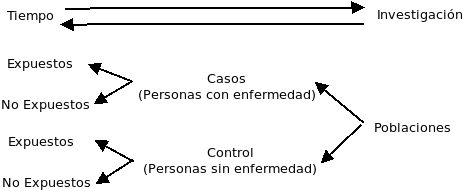
\includegraphics[width=0.5\columnwidth]{A.imagenes/ACV-EPI-CasosControles}
	\caption{Ejemplo de intervención en estudio de casos-controles.}
\end{figure}
\subsubsection{Selección de casos y controles}
Un estudio de casos-controles comienza con la selección de casos. Estos representarían todos los casos en un grupo poblacional espcífico. Los casos son seleccionados en base a la enfermedad y no a la exposición. Los controles son personas sin la enfermedad. Un aspecto fundamental y exigente de los estudios basados en casos-controles es encontrar una manera de coste apropiado para identificar y enrolar sujetos controles para mostrar la prevalencia de la exposición en la población que genera los casos. Además, la elección de controles y casos debe no estar influenciada por el estado de exposición, que debe ser determinado de la misma manera en ambos. No es necesario ser inclusivo, de hecho puede restringirse a cualquier subgrupo específico.

Los controles representan presonas quienes habrían estado designados al estudio como casos si hubieran contraído la enfermedad. Idealmente, los estudios de caso-control utiliza nuevos casos (incidentes) para evitar la dificultad de separar factores que intervienen en la causalidad y supervivencia (o recuperación), aunque los estudios han sido, con frecuencia, conducidos usando datos de prevalencia (por ejemplo, estudios de caso-control de malformaciones genéticas). Los estudios de casos-controles estiman el riesgo relativo de enfermedad, pero no determinan de forma absoluta la incidencia de enfermedad.
\subsubsection{Exposición}
Un aspecto importante de los estudios de caso-control es la determinación de comienzo y duración de la exposición para casos y controles. En el diseño de casos-controles, el estado de exposición de los casos es normalmente determinado después del desarrollo de la enfermedad (datos retrospectivos) y normalmente por cuestionarios directos de afectados o familiares y amigos. Las respuestas de los informantes puede estar influenciada por el conocimiento de la hipótesis bajo investigación o la experiencia propia de la enfermedad.

La exposición se determina a veces por parámetros bioquímicos (por ejemplo, plomo en sangre o cadmio en orina), los cuales pueden no representar la relevancia de exposiciones pasadas. Por ejemplo, el plomo en sangre a los 6 años no es un buen indicador de la exposición a los 1 ó 2 años, edades con gran sensibilidad al plomo. Este problema puede ser evitado si la exposición puede ser estimada por un sistema establecido de registro (guardado de resultado de test de sangre rutinario) o si los estudios caso-control son llevados a cabo de forma prospectiva, de manera que los datos son recogidos antes del desarrollo de la enfermedad.
\subsubsection{\textit{Odds ratio} o proporción de razones}
La asociación de exposición y enfermedad (riesgo relativo) en un estudio de caso-control se mide mediante el cálculo de <<\textit{odds ratio}>> (OR) que es la proporción de las razones de exposición entra la razones de los controles. Las \textit{odds ratio} es similar a la proporción de riesgo, especialmente si la enfermedad es rara. Para la proporción de razones sea una buena aproximación, los casos y los controles deben ser representativos de la población general con respecto a la exposición. Sin embargo, debido a que la incidencia de la enfermedad es desconocida, el riesgo absoluto no puede ser calculado. Una proporción de razones ha de ser acompañado de un intervalo de confianza sobre el punto estimado.
\begin{table}[H]
	\centering
	\begin{tabular}{
			>{\columncolor[HTML]{000000}}l 
			>{\columncolor[HTML]{000000}}l lll}
		{\color[HTML]{FFFFFF} } & {\color[HTML]{FFFFFF} } & \multicolumn{2}{l}{\cellcolor[HTML]{000000}{\color[HTML]{FFFFFF} Exposición}} &  \\
		{\color[HTML]{FFFFFF} } & {\color[HTML]{FFFFFF} } & \cellcolor[HTML]{000000}{\color[HTML]{FFFFFF} Sí} & \cellcolor[HTML]{000000}{\color[HTML]{FFFFFF} No} &  \\
		\cellcolor[HTML]{000000}{\color[HTML]{FFFFFF} } & {\color[HTML]{FFFFFF} Sí} & A & B &  \\
		\multirow{-2}{*}{\cellcolor[HTML]{000000}{\color[HTML]{FFFFFF} Enfermedad}} & {\color[HTML]{FFFFFF} No} & \cellcolor[HTML]{DAE8FC}C & \cellcolor[HTML]{DAE8FC}D &
	\end{tabular}
	\caption[Cuadro de Punnet u \textit{Odds ratio}]{Cuadro de Punnet u \textit{Odds ratio}: en esta tabla se clasifican los distintos casos por su grado de exposición.}
\end{table}
\begin{center}
	\begin{equation}
		OR = \dfrac{A\cdot D}{B\cdot C}
	\end{equation}
	\captionof{Ecuacion}[Ecuación de \textit{Odds Ratio}]{Ecuación de \textit{Odds ratio}, leida como la posiblidad de un sujeto expuesto a desarrollar la enfermedad.}
\end{center}
\subsection{Estudios de cohortes}
Los estudios de cohortes comienzan con un grupo de presonas libres de la enfermedad y que son clasificados en subgrupos de acuerdo a la exposición a una causa potencial de enfermedad o resultado. Las variables de interés son especificados y medidos y la cohorte entera es seguida para observar como el ulterior desarrollo de nuevos casos de enfermedad (u otro resultado) difiere entre grupos con y sin exposición. Dado que los datos de exposición y enfermedad se refieren a diferentes puntos en el tiempo, los estudios de cohortes son longitudinales. Los estudios de cohortes son estudios de futuro, término confuso que puede ser evitado, ya que se refiere al momento de recabación de datos, no a la relación exposición-efectos, pudiendo haber estudios retrospectivos o de futuro.

Los estudios de cohorte proveen la mejor información sobre la causa de la enfermedad y la medida más directa del riesgo de contraer la enfermedad. Aunque conceptualmente simples, son muy complejos y pueden requerir largos periodos de tiempo de seguimiento desde que la enfermedad puede ocurrir un tiempo largo de exposición. Muchas exposiciones son investigadas durante largos periodos en la naturaleza y la precisa información sobre ellas requiere largos periodos de recogida de datos.

En situaciones con repetidas y puntuales exposiciones, la relación causa-efecto para efectos puntuales puede ser obvio, pero los estudios de cohortes son también usados para investigar efectos tardíos o crónicos. Como un estudio de cohortes empieza con gente expuesta y no expuesta, la dificultad de medida o el hallar datos existentes en exposiciones en gran medida determina la viabilidad de realización de estos. Si la enfermedad es rara en grupos expuestos y no expuestos puede provocar también problemas en la obtención en grupos suficientemente grandes de estudio.

El coste de un estudio de cohortes puede ser reducido usando fuentes rutinarias de información sobre mortalidad y morbilidad, como registros de enfermedades o registros nacionales de muertes como parte del seguimiento. Un tipo especial de estudios de cohortes con los estudios de gemelos, donde el factor de variación genética (entre gente expuesta y no expuesta a un factor particular) puede ser eliminado. Como estudios ha provisto de fuertes evidencias para una variedad de relaciones causa-efecto para enfermedades crónicas.
\begin{figure}[H]
	\centering
	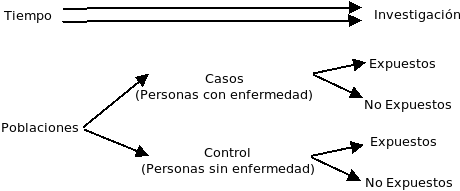
\includegraphics[width=0.5\columnwidth]{A.imagenes/ACV-EPI-Cohortes}
	\caption{Ejemplo de intervención en estudio de cohortes.}
\end{figure}
\subsubsection{Estudios de cohortes históricos}
Los costes pueden ser reducidos usando cohortes históricas (identificadas en base a crónicas de exposición previas). Se llaman así porque toda exposición y efecto (enfermedad) ha sido recogida antes del comienzo del estudio actual. Este orden de diseño es muy común para estudios que relacionan cáncer y exposiciones laborales.
\subsubsection{Estudios caso-control integrados}
El diseño de estudios caso-control integrados hace menos caros a los estudios de cohortes. Los casos y los controles son ambos escogidos de una cohorte definida para el cual alguna información sobre exposición y factores de riesgo está ya disponible. Información adicional de nuevos casos y controles, particularmente seleccionados para el estudio son recogidos y analizados. Estos diseños son particularmente útiles cuando la medida de la exposición es cara.
\section{Epidemiología experimental}
La intervención o experimentación implica intenta cambiar una variable en uno o más grupos de personas. Esto puede significar la eliminación de un factor dietético que se piense que provoca alergia, o la prueba de un nuevo tratamiento sobre un nuevo tratamiento sobre un grupo seleccionado de pacientes. Los efectos de una intervención han de ser medidos mediante comparación de resultados con el grupo control. Puesto que las intervenciones están estrictamente reguladas por los estudios de protocolo, las consideraciones éticas son de importancia capital en el diseño de estudios. Por ejemplo, ningún paciente debe serle denegado el tratamiento apropiado como resultado de la participación en un experimento, y este debe ser testado a la luz del conocimiento actual. El consentimiento informado es requerido en todos los casos.
\subsection{Estudios clínicos}
Un estudio clínico es un experimento epidemiológico diseñado para estudiar los efectos de una intervención particular, normalmente un tratamiento para una enfermedad específica. Los sujetos en el estudio poblacional son aleatoriamente asignados a grupos control o de intervención, y los resultados son calculados por comparación. Para asegurar que los grupos que están siendo comparados son equivalentes, los pacientes son asignados aleatoriamente. Si la selección inicial y la aleatorización se hicieron adecuadamente, los grupos control y de tratamiento serán comparables al inicio de la investigación; cualquier diferencia entre grupos son acontecimientos no afectados por sesgos conscientes o inconscientes de los investigadores.
\begin{figure}[H]
	\centering
	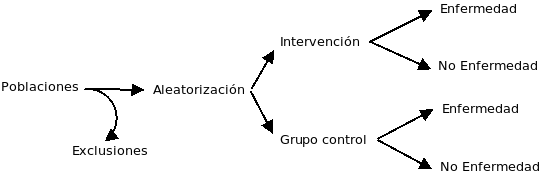
\includegraphics[width=0.5\columnwidth]{A.imagenes/ACV-EPI-EstudioClinico}
	\caption{Ejemplo de intervención en estudio clínico.}
\end{figure}
\subsection{Estudios de campo}
Los estudios de campo implica a la población sana pero presupuesta a estar en riesgo. La recolección de datos se toma <<en el campo>>, normalmente entre personas no institucionalizadasde la población general. Entonces los sujetos están libres de enfermedades y el propósito es prevenir las enfermedades que pueden ocurrir con relativamente baja frecuencia. Suelen ser logisticamente complejos y suponen un esfuerzo costoso (un ejemplo fue la vacuna frente a la polio de Salk, con un millón de infantes vacuandos).

Los estudios de campo pueden ser usados para evaluar intervenciones apuntando a reducir la exposición sin necesariamente medir los sucesos de los efectos de salud. Cada estudio de intervención puede hacerse en menor escala y con menor coste así como no implicar un largo seguimiento o medida de los resultados de enfermedades.
\subsection{Pruebas comunitarias}
En este tipo de experimentos, el grupo de tratamiento son comunidades antes que individuos. Esto es particularmente apropiado para enfermedades que son influenciadas por las condiciones sociales y para esfuerzos de prevención sobre grupos de comportamiento.
\subsubsection{Limitaciones}
Una limitación de estos estudios es que sólo un pequeño número de comunidades puede ser incluido y la distribución aleatoria de las comunidades no es normalmente viable. Otros métodos son requeridos para asegurar que cualquier diferencia encontrada al finalizar el estudio pueden ser atribuidas a la intervención preferiblemente que a diferencias inherentes entre comunidades. Además es difícil aislar comunidades donde la intervención tiene lugar frente a cambios sociales generales que pueden estar ocurriendo. Las limitaciones del diseño, especialmente frente a inesperadamente largos, los factores de riesgo favorables cambian en sitios control, siendo dificil calcularlos. Como consecuencia, las conclusiones definitivas sobre la efectividad global de los intentos internacionales no son siempre positivos.
\begin{table}[H]
	\centering
	\begin{tabular}{M{2.15cm}N{2.15cm}N{1.8cm}N{2cm}N{2.5cm}N{1.8cm}N{2cm}}
		\rowcolor{black}\textcolor{white}{\textbf{Estudios}}&\textcolor{white}{\textbf{Descriptivo}}&\textcolor{white}{\textbf{Analíticos}}&\textcolor{white}{\textbf{Ecológicos}}&\textcolor{white}{\textbf{Transversales}}&\textcolor{white}{\textbf{Caso-Control}}&\textcolor{white}{\textbf{Cohortes}}\\
		Unidad de estudio&---&---&Población&Individuos&Individuos&Individuos\\
		Enfermedades raras&-&-&+&-&+&-\\
		\rowcolor{hiperlightgray}Causas raras&-&-&+&-&-&+\\
		Múltiples efectos de causa&-&-&+&+&-&+\\
		\rowcolor{hiperlightgray}Multiples exposiciones y determinantes&-&-&+&+&+&+\\
		Medidas relacionadas con tiempo&-&-&+&-&+&+\\
		\rowcolor{hiperlightgray}Medida directa incidencia&-&-&-&-&+&+\\
		Investigaciones largo tiempo&-&-&-&-&+&-\\
		\hline
	\end{tabular}
	\caption{Aplicaciones de los estudios epidemiológicos.}
\end{table}
\section{Errores potenciales en estudios epidemiológicos}
La investigación  aspira a proveer de medidas exactas de la incidencia de enfermedades u otro resultado en salud. Sin embargo, hay muchas posibilidades de errror en la medida que debe ser minimizado y calculado aquél que no puede ser eliminado. Los tipos de error:
\begin{itemize}[itemsep=0pt,parsep=0pt,topsep=0pt,partopsep=0pt]
	\item \textbf{Error aleatorio}: ocasionados por variaciones en la medida de la muestra, debido únicamente al azar, determinando un valor que diverge del real, causando inexactitud en la medida. El error aleatorio nunca puede ser eliminado desde que se estudia una muestra de la población. Son tres los tipos, no pudiéndose eliminar por un estudio sobre una muestra:
	\begin{itemize}[itemsep=0pt,parsep=0pt,topsep=0pt,partopsep=0pt]
		\item \textbf{Variación biológica individual}: Siempre ocurre y la medida no es perfecta.
		\item\textbf{Error de muestreo}: causado por el hecho de que una pequeña muestra no es representativa de todas las variables poblacionales. La mejor forma de reducirla es aumentar el tamaño del estudio.
		\item\textbf{Error de medida}: el error de medida puede ser reducido por severos protocolos, y haciendo medidas individuales tan precisas como sean posibles. Es preciso conocer el método de medida usado y los errores que pueden producir. Los laboratorios han de contar con procedimientos de control de calidad (exactitud y precisión de medidas).
	\end{itemize}
	\item\textbf{Tamaño de muestra}: La muestra debe ser lo suficientemente grande para tener el suficiente poder estadístico para detectar las diferencias importantes estimadas. El tamaño al final se determina por consideraciones logísticas y financieras, y ha de de hacerse un compromiso entre los costes y el tamaño de la muestra. La siguiente información es necesaria antes de que los cálculos se hagan:
	\begin{itemize}[itemsep=0pt,parsep=0pt,topsep=0pt,partopsep=0pt]
		\item Requiere un nivel de significación estadística con la capacidad de detectar la diferencia.
		\item Nivel de error aceptable o se arriesga a perder el efecto real.
		\item Magnitud del efecto bajo investigación.
		\item Tamaño relativo de los grupos a comparar.
	\end{itemize}
	\item\textbf{Precisión}: la precisión del estudio puede ser también mejorada asegurandose de que los grupos son del tamaño relativo apropiado. Este es frecuentemente un asunto que afecta a estudios de caso-control cuando se requiere una decisión sobre el número de controles para cada caso. Si no es posible, ser definitivo sobre el ratio ideal de controles sobre casos, entonces depende de los costes relativos de recopilar casos y controles. En general, sin embargo, podría haber un pequeño punto donde se puede tener más cuatro controles por caso. Es importante asegurar que hay la suficiente similitud entre casos y controles cuando los datos son analizados por edad, grupo, o clase social, $\dots$ Si hay más casos, y solo unos pocos controles, el estudio podría no tener en cuenta la confusión por ciertos factores.
	\item\textbf{Error sistemático}: el error o sesgo sistemático acontece cuando los resultados difieren de una manera sistemática de los valores reales. Un estudio con un pequeño error sistemático es altamente exacto. La exactitud no se ve afectada por el tamaño de la muestra. Las posibles fuentes de error sistemático son muchos y variados, siendo los principales:
	\begin{itemize}[itemsep=0pt,parsep=0pt,topsep=0pt,partopsep=0pt]
		\item \textbf{Sesgo o error de selección}: ocurre cuando hay una diferencia sistemática entre las características de la gente seleccionada para un estudio y las características de quienes no están. Un origen obvio del sesgo ocurre cuando los participantes se seleccionan así mismos para un estudio, o porque ellos están enfermos o porque están preocupados por una exposición. Si los individuos entran o permanecen en un estudio que tiene diferentes características de aquellos quienes no fueron seleccionados inicialmente, o quien salió antes de terminar, el resultado es una estimación parcial de la asociación entre exposición y resultado. Un importante sesgo de selección se introduce cuando la enfermedad o el factor bajo investigación hace a la gente no útil para el estudio (trabajadores que abandonan el trabajo por molestias provocadas por la exposición). En cada estudio epidemiológico necesita un diseño que cuente con el sesgo.
		\item \textbf{Sesgo de medida o clasificación}:
	\end{itemize}
\end{itemize}